%
% BAYESIAN SKYLINE PLOT
%

\begin{frame}
\frametitle{The Bayesian skyline plot (Drummond {\it et al}, 2005)}

\begin{columns}

\column{0.35\textwidth}

The Bayesian skyline plot estimates a demographic function that has a certain fixed number of steps (in this example 15) and then integrates over all possible positions of the break points, and population sizes within each epoch.

\column{0.65\textwidth}

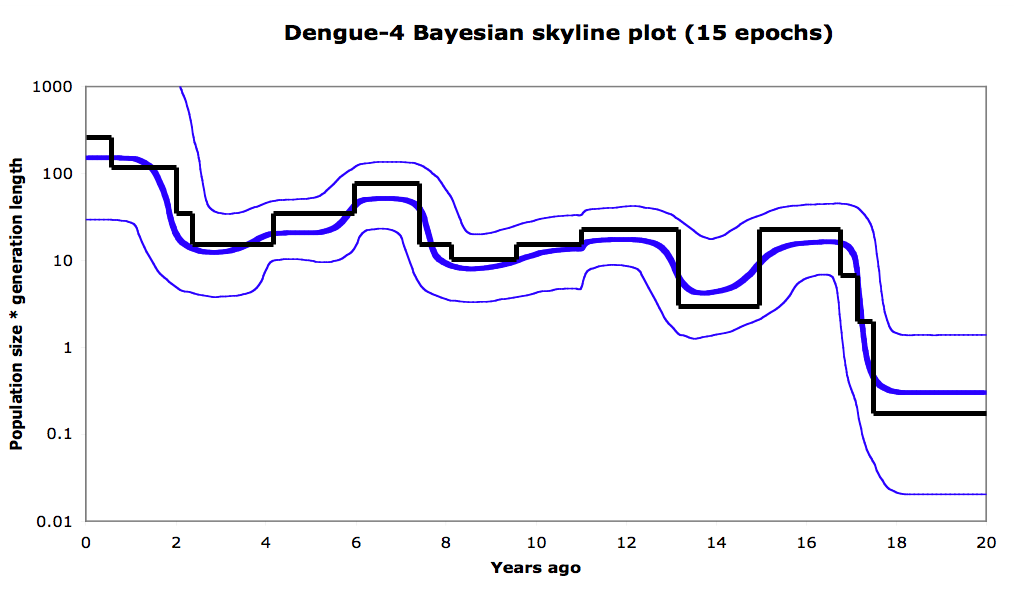
\includegraphics[width=\textwidth]{../images/dengueBSPLog}

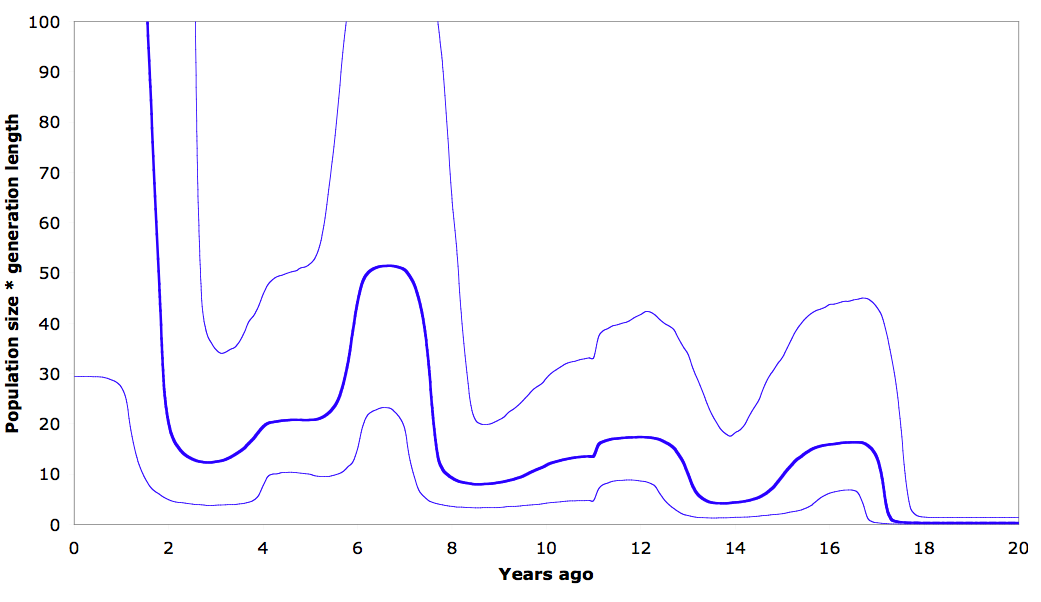
\includegraphics[width=\textwidth]{../images/dengueBSP}

\end{columns}
\end{frame}

% EBSP SLIDES
\begin{frame}
\frametitle{Detecting evolutionary bottlenecks using EBSP}
%\framesubtitle{480 contemporaneous samples from a single locus}
\center{%

480 contemporaneous samples from a single locus

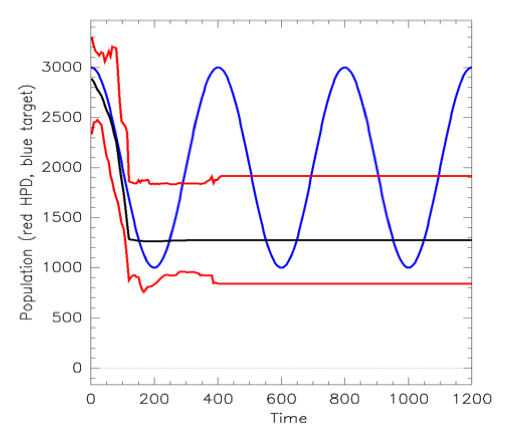
\includegraphics[width=0.6\textwidth]{../images/EBSP_detectingBottlenecks1}%

}
\end{frame}

\begin{frame}
\frametitle{Detecting evolutionary bottlenecks using EBSP}
%\framesubtitle{16 contemporaneous samples from each of 32 loci}
\center{%

16 contemporaneous samples from each of 32 loci

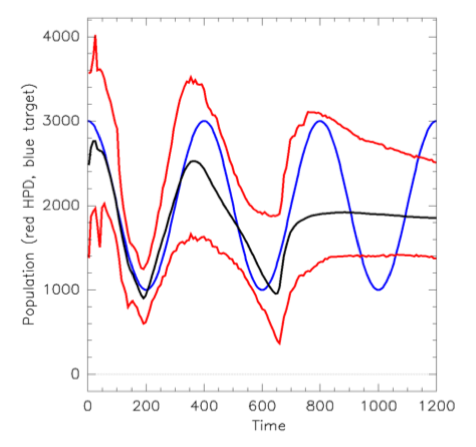
\includegraphics[width=0.6\textwidth]{../images/EBSP_detectingBottlenecks2}%

}
\end{frame}

\begin{frame}
\frametitle{Detecting evolutionary bottlenecks using EBSP}
%\framesubtitle{480 samples sampled through time ($t=[0-1000]$) from a single locus}
\center{%

480 samples sampled through time from a single locus

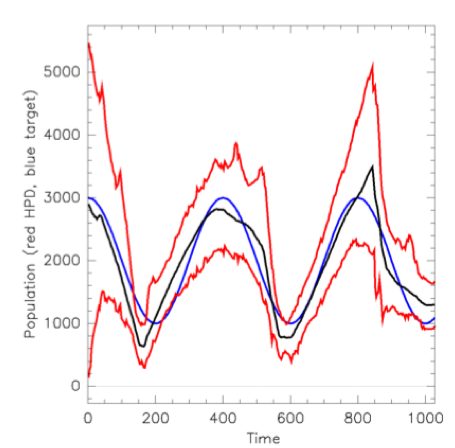
\includegraphics[width=0.6\textwidth]{../images/EBSP_detectingBottlenecks3}%

}
\end{frame}

\begin{frame}
\frametitle{The population dynamics of genetic diversity in Influenza A}
\framesubtitle{Rambaut {\it et al} (2008) {\it Nature} {\bf 453}:615-620}
\begin{centering}%
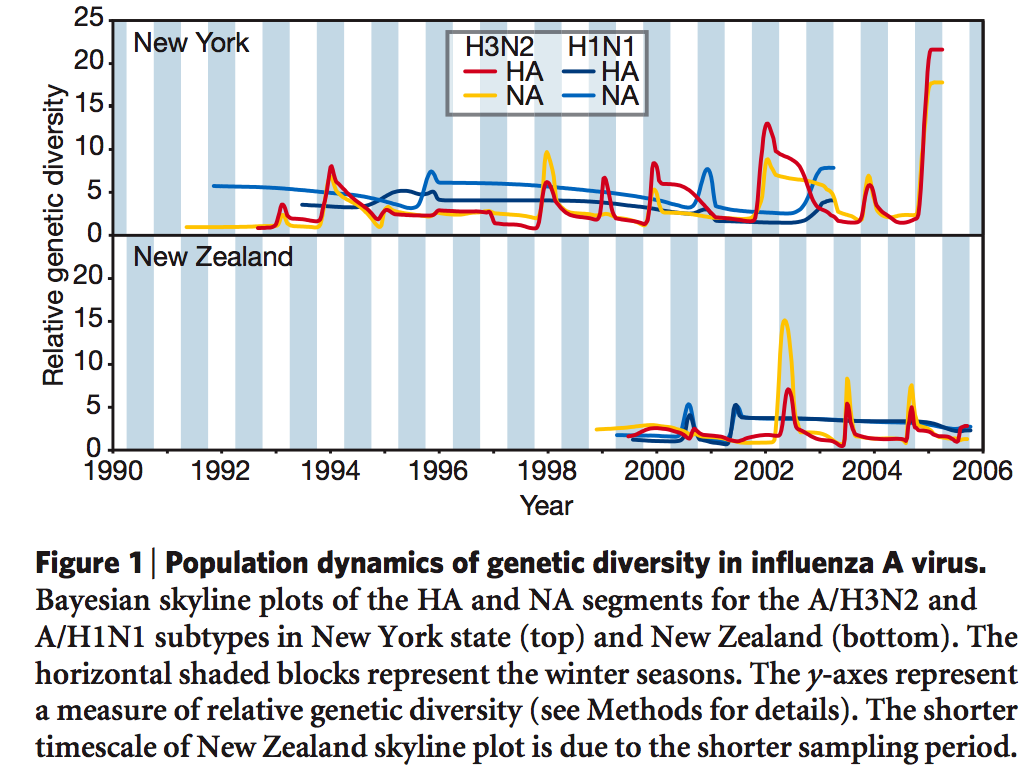
\includegraphics[width=0.8\textwidth]{../images/bsp/Rambaut2008_Figure1}%
\par%
\end{centering}%
\end{frame}

%\begin{frame}
%\frametitle{Validating the Bayesian skyline plot}
%\begin{centering}%
%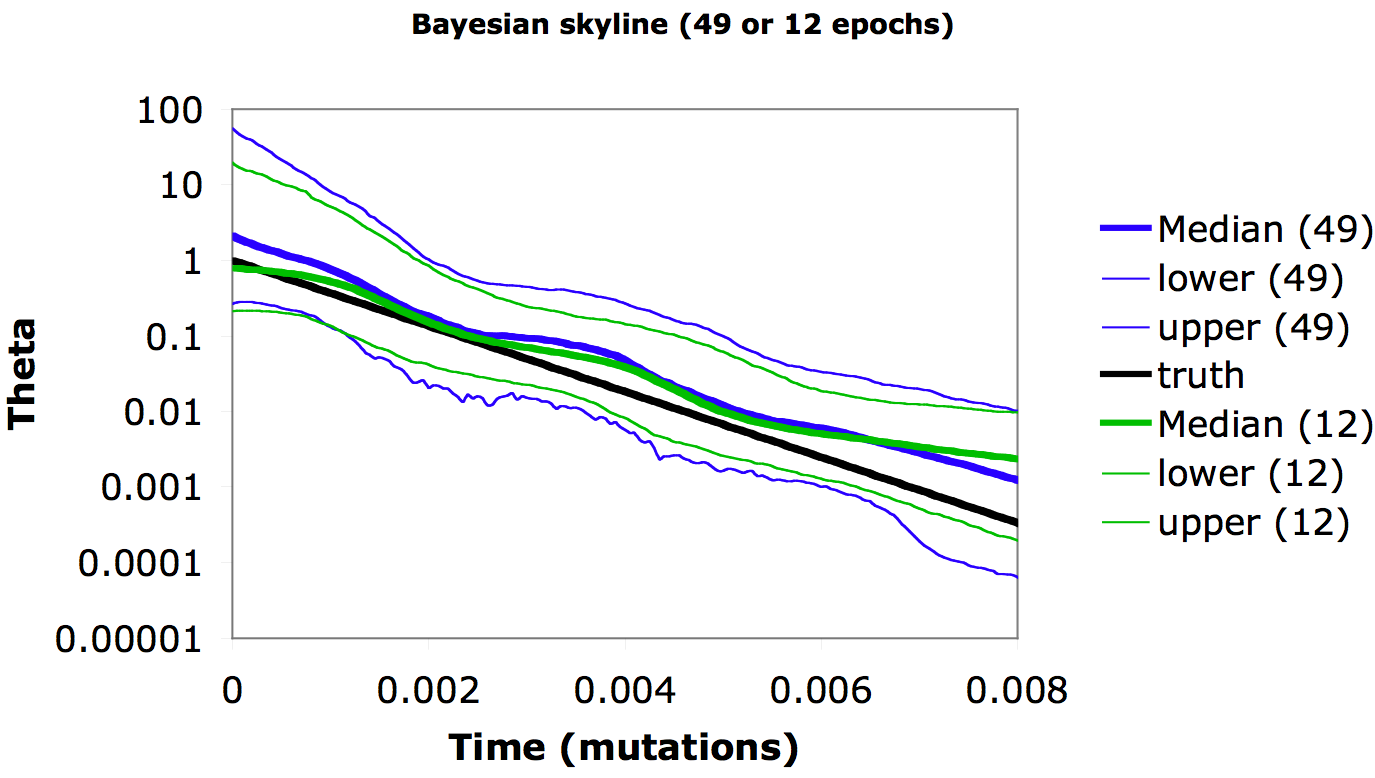
\includegraphics[width=1.05\textwidth]{validatingBSP}%
%\par%
%\end{centering}%
%\end{frame}

\begin{frame}
\frametitle{Comparison of BSP to parametric coalescent model}
\framesubtitle{Hepatitis C in Egypt}
\begin{centering}%
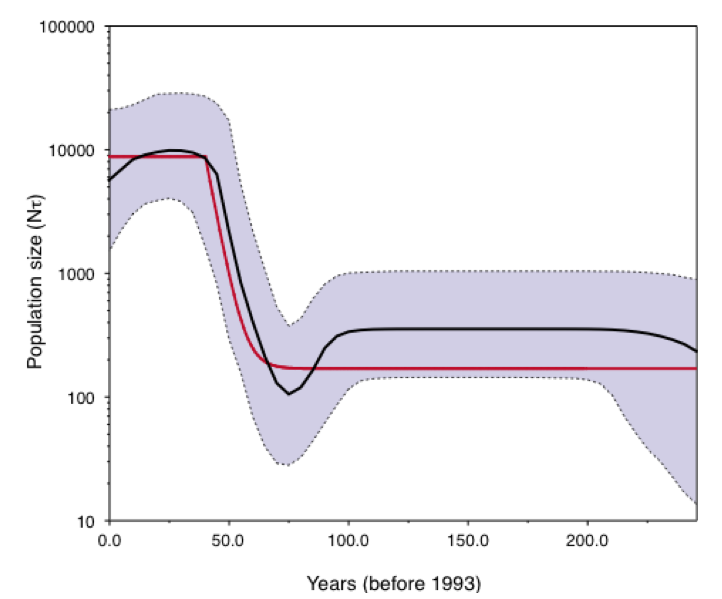
\includegraphics[width=0.8\textwidth]{../images/hepatitisC/HCV_parametricVersusBSP}%
\par%
\end{centering}%
\end{frame}

%\begin{frame}
%\frametitle{Modeling complex demographic history}
%\framesubtitle{Dengue 4 in Puerto Rico}
%\begin{centering}%
%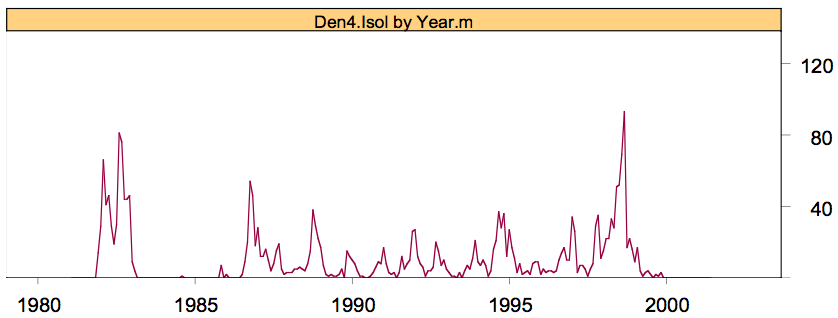
\includegraphics[width=\textwidth]{../images/dengue4_isolatesByYear}%
%\par%
%\end{centering}%
%
%\begin{itemize}
%\item $N(t) = N_0\exp(-rt)$
%  \begin{itemize}
%  \item log marginal likelihood = -10566.421
%  \end{itemize}
%\item $N(t) = \mbox{scaled-translated case data}$
%  \begin{itemize}
%  \item log marginal likelihood = -10478.572
%  \end{itemize}
%\end{itemize}
%\end{frame}
%
%\begin{frame}
%\frametitle{Comparing BSP to incidence data}
%\framesubtitle{Dengue 4 in Puerto Rico}
%\begin{centering}%
%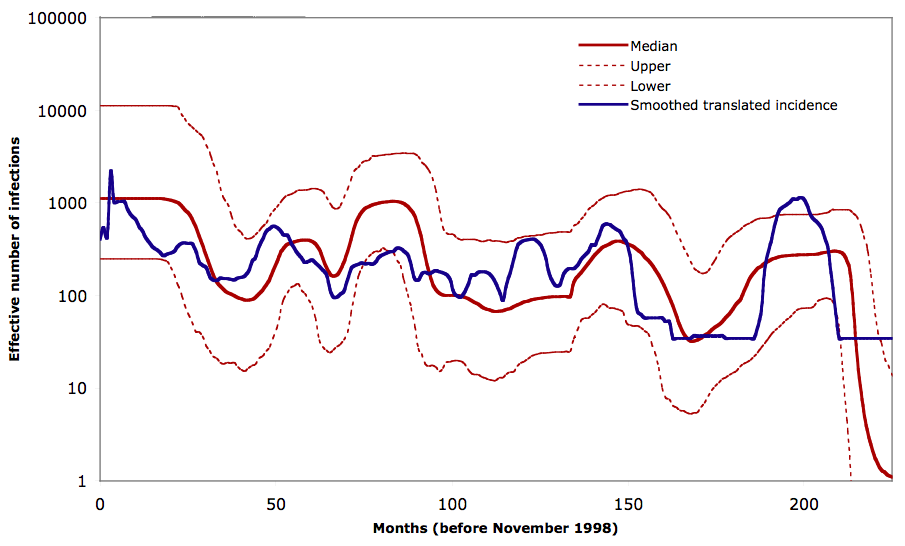
\includegraphics[width=\textwidth]{../images/dengue4_BSP}%
%\par%
%\end{centering}%
%\end{frame}
